\documentclass{vkr}
\usepackage[english, russian]{babel} % переносы
\usepackage{graphicx} % для вставки картинок
\graphicspath{{images/}} % путь к изображениям
\usepackage[hidelinks]{hyperref}
\usepackage{float} % определяет метод H для рисунка с переносом на следующую страницу, ели не помещается
\usepackage{pdflscape}
\addto{\captionsrussian}{\renewcommand{\refname}{СПИСОК ИСПОЛЬЗОВАННЫХ ИСТОЧНИКОВ}}
\usepackage{xltabular} % для вставки таблиц
\usepackage{makecell}
\renewcommand\theadfont{} % шрифт в /thead
\usepackage{array} % для определения новых типов столбцов таблиц
\newcolumntype{T}{>{\centering\arraybackslash}X} % новый тип столбца T - автоматическая ширина столбца с выравниванием по центру
\newcolumntype{R}{>{\raggedleft\arraybackslash}X} % новый тип столбца R - автоматическая ширина столбца с выравниванием по правому краю
\newcolumntype{C}[1]{>{\centering\let\newline\\\arraybackslash\hspace{0pt}}m{#1}} % новый тип столбца C - фиксированная ширина столбца с выравниванием по центру
\newcolumntype{r}[1]{>{\raggedleft\arraybackslash}p{#1}} % новый тип столбца r - фиксированная ширина столбца с выравниванием по правому краю
\newcommand{\centrow}{\centering\arraybackslash} % командой \centrow можно центрировать одну ячейку (заголовок) в столбце типа X или p, оставив в оcтальных ячейках другой тип выравнивания
\newcommand{\finishhead}{\endhead\hline\endlastfoot}
\newcommand{\continuecaption}[1]{\captionsetup{labelformat=empty} \caption[]{#1}\\ \hline }
\usepackage{etoolbox}
\AtBeginEnvironment{xltabular}{\refstepcounter{tablecnt}} % подсчет таблиц xltabular, обычные таблицы подсчитываются в классе

\usepackage[tableposition=top]{caption} % подпись таблицы вверху
\captionsetup{strut=off}
\setlength{\intextsep}{0pt} % Vertical space above & below [h] floats
\setlength{\textfloatsep}{0pt} % Vertical space below (above) [t] ([b]) floats
\DeclareCaptionLabelFormat{gostfigure}{Рисунок #2} %подпись рисунка
\DeclareCaptionLabelFormat{gosttable}{Таблица #2} %подпись таблицы
\DeclareCaptionLabelSeparator{gost}{~--~} %разделитель в рисунках и таблицах
\captionsetup{labelsep=gost}
\captionsetup[figure]{aboveskip=10pt,belowskip=4mm,justification=centering,labelformat=gostfigure} % настройка подписи рисунка
\captionsetup[table]{font={stretch=1.41},skip=0pt,belowskip=0pt,aboveskip=8.5pt,singlelinecheck=off,labelformat=gosttable} % настройка подписи таблицы

\setlength{\LTpre}{8mm} % отступ сверху таблицы
\setlength{\LTpost}{6mm} % отступ снизу таблицы

\usepackage{enumitem}
\setlist{nolistsep,wide=\parindent,itemindent=*} % отступы вокруг списков, выравнивание с учетом разделителя

\usepackage{color} %% это для отображения цвета в коде
\usepackage{listings} %% листинги кода
\setmonofont[Scale=0.7]{Verdana} % моноширный шрифт для листинга

\definecolor{codegreen}{rgb}{0,0.6,0}
\definecolor{codegray}{rgb}{0.5,0.5,0.5}
\definecolor{codepurple}{rgb}{0.58,0,0.82}

\lstset{ %
language=C,                 % выбор языка для подсветки (здесь это С)
numbers=left,               % где поставить нумерацию строк (слева\справа)
numberstyle=\tiny,           % размер шрифта для номеров строк
stepnumber=1,                   % размер шага между двумя номерами строк
numbersep=5pt,                % как далеко отстоят номера строк от подсвечиваемого кода
commentstyle=\color{codegreen},
keywordstyle=\color{magenta},
numberstyle=\tiny\color{codegray},
stringstyle=\color{codepurple},
basicstyle=\linespread{0.95}\ttfamily,
backgroundcolor=\color{white}, % цвет фона подсветки - используем \usepackage{color}
showspaces=false,            % показывать или нет пробелы специальными отступами
showstringspaces=false,      % показывать или нет пробелы в строках
showtabs=false,             % показывать или нет табуляцию в строках
frame=single,              % рисовать рамку вокруг кода
tabsize=2,                 % размер табуляции по умолчанию равен 2 пробелам
captionpos=t,              % позиция заголовка вверху [t] или внизу [b] 
breaklines=true,           % автоматически переносить строки (да\нет)
breakatwhitespace=false, % переносить строки только если есть пробел
escapeinside={\%*}{*)}   % если нужно добавить комментарии в коде
}

\makeatletter % чтобы допускались русские комментарии в листингах
\lst@InputCatcodes
\def\lst@DefEC{%
 \lst@CCECUse \lst@ProcessLetter
  ^^80^^81^^82^^83^^84^^85^^86^^87^^88^^89^^8a^^8b^^8c^^8d^^8e^^8f%
  ^^90^^91^^92^^93^^94^^95^^96^^97^^98^^99^^9a^^9b^^9c^^9d^^9e^^9f%
  ^^a0^^a1^^a2^^a3^^a4^^a5^^a6^^a7^^a8^^a9^^aa^^ab^^ac^^ad^^ae^^af%
  ^^b0^^b1^^b2^^b3^^b4^^b5^^b6^^b7^^b8^^b9^^ba^^bb^^bc^^bd^^be^^bf%
  ^^c0^^c1^^c2^^c3^^c4^^c5^^c6^^c7^^c8^^c9^^ca^^cb^^cc^^cd^^ce^^cf%
  ^^d0^^d1^^d2^^d3^^d4^^d5^^d6^^d7^^d8^^d9^^da^^db^^dc^^dd^^de^^df%
  ^^e0^^e1^^e2^^e3^^e4^^e5^^e6^^e7^^e8^^e9^^ea^^eb^^ec^^ed^^ee^^ef%
  ^^f0^^f1^^f2^^f3^^f4^^f5^^f6^^f7^^f8^^f9^^fa^^fb^^fc^^fd^^fe^^ff%
  ^^^^20ac^^^^0153^^^^0152%
  % Basic Cyrillic alphabet coverage
  ^^^^0410^^^^0411^^^^0412^^^^0413^^^^0414^^^^0415^^^^0416^^^^0417%
  ^^^^0418^^^^0419^^^^041a^^^^041b^^^^041c^^^^041d^^^^041e^^^^041f%
  ^^^^0420^^^^0421^^^^0422^^^^0423^^^^0424^^^^0425^^^^0426^^^^0427%
  ^^^^0428^^^^0429^^^^042a^^^^042b^^^^042c^^^^042d^^^^042e^^^^042f%
  ^^^^0430^^^^0431^^^^0432^^^^0433^^^^0434^^^^0435^^^^0436^^^^0437%
  ^^^^0438^^^^0439^^^^043a^^^^043b^^^^043c^^^^043d^^^^043e^^^^043f%
  ^^^^0440^^^^0441^^^^0442^^^^0443^^^^0444^^^^0445^^^^0446^^^^0447%
  ^^^^0448^^^^0449^^^^044a^^^^044b^^^^044c^^^^044d^^^^044e^^^^044f%
  ^^^^0401^^^^0451%
  %%%
  ^^00}
\lst@RestoreCatcodes
\makeatother


% Режим шаблона (должен быть включен один из трех)
\ВКРtrue
%\Практикаtrue
%\Курсоваяtrue

\newcommand{\Дисциплина}{<<Проектирование и архитектура программных систем>>} % для курсовой
\newcommand{\КодСпециальности}{09.03.04} % Курсовая
\newcommand{\Специальность}{Программная инженерия} % Курсовая
\newcommand{\Тема}{Бизнес-проект «Закрытый корпоративный мессенджер.} % ВКР Курсовая
\newcommand{\ТемаВтораяСтрока}{Разработка модели данных»}
\newcommand{\ГдеПроводитсяПрактика}{ООО "МЦОБ.Онлайн-Сервисы"} % для практики
\newcommand{\РуководительПрактПредпр}{Куркина А. В.} % для практики
\newcommand{\ДолжнРуководительПрактПредпр}{директор} % для практики
\newcommand{\РуководительПрактУнивер}{Чаплыгин А. А.} % для практики
\newcommand{\ДолжнРуководительПрактУнивер}{к.т.н. доцент} % для практики
\newcommand{\Автор}{М.В. Заболоцкий}
\newcommand{\АвторРод}{Заболоцкий М.В.}
\newcommand{\АвторПолностьюРод}{Заболоцкого Максима Валерьевича} % для практики
\newcommand{\Шифр}{21-06-0096}
\newcommand{\Курс}{4} % для практики
\newcommand{\Группа}{ПО-11б}
\newcommand{\Руководитель}{А. А. Чаплыгин} % для ВКР и курсовой
\newcommand{\Нормоконтроль}{А. А. Чаплыгин} % для ВКР
\newcommand{\ЗавКаф}{А. В. Малышев} % для ВКР
\newcommand{\ДатаПриказа}{«04» апреля 2025~г.} % для ВКР
\newcommand{\НомерПриказа}{1696-с} % для ВКР
\newcommand{\СрокПредоставления}{«13» июня 2023~г.} % для ВКР, курсового

\begin{document}
	\maketitle
	\ifПрактика{}\else{
		\newpage
\begin{center}
\large\textbf{Минобрнауки России}

\large\textbf{Юго-Западный государственный университет}
\vskip 1em
\normalsize{Кафедра программной инженерии}
\vskip 1em
\ifВКР{
        \begin{flushright}
        \begin{tabular}{p{.4\textwidth}}
        \centrow УТВЕРЖДАЮ: \\
        \centrow Заведующий кафедрой \\
        \hrulefill \\
        \setarstrut{\footnotesize}
        \centrow\footnotesize{(подпись, инициалы, фамилия)}\\
        \restorearstrut
        «\underline{\hspace{1cm}}»
        \underline{\hspace{3cm}}
        20\underline{\hspace{1cm}} г.\\
        \end{tabular}
        \end{flushright}
        }\fi
\end{center}
\vspace{1em}
  \begin{center}
  \large
\ifВКР{
ЗАДАНИЕ НА ВЫПУСКНУЮ КВАЛИФИКАЦИОННУЮ РАБОТУ
  ПО ПРОГРАММЕ БАКАЛАВРИАТА}
  \else
ЗАДАНИЕ НА КУРСОВУЮ РАБОТУ (ПРОЕКТ)
\fi
\normalsize
  \end{center}
\vspace{1em}
{\parindent0pt
  Студента \АвторРод, шифр\ \Шифр, группа \Группа
  
1. Тема «\Тема\ \ТемаВтораяСтрока»
\ifВКР{
утверждена приказом ректора ЮЗГУ от \ДатаПриказа\ № \НомерПриказа
}\fi.

2. Срок предоставления работы к защите \СрокПредоставления

3. Исходные данные для создания программной системы:

3.1. Перечень решаемых задач:}

\renewcommand\labelenumi{\theenumi)}

\begin{enumerate}
	\item проанализировать требования к данным корпоративного мессенджера;
	\item разработать концептуальную, логическую и физическую модели данных системы;
	\item спроектировать реляционную схему БД с учётом бизнес-процессов обмена сообщениями;
	\item реализовать и протестировать модель данных в СУБД SQLite.
\end{enumerate}

{\parindent0pt
	3.2. Входные данные и требуемые результаты для программы:}

\begin{enumerate}
	\item Входными данными для системы являются: учетные данные пользователей (логин/пароль); текстовые сообщения пользователей; прикрепляемые файлы (изображения, документы); запросы на создание/управление группами и их участниками; параметры поиска по истории сообщений.
	
	\item Выходными данными системы являются: отправленные сообщения в чатах (общих, групповых, приватных); уведомления о новых сообщениях и событиях; списки доступных групп и пользователей; результаты поиска по сообщениям; статистика активности пользователей; файлы, загруженные пользователями.
\end{enumerate}

{\parindent0pt

  4. Содержание работы (по разделам):
  
  4.1. Введение.
  
  4.1. Анализ предметной области.
  
4.2. Техническое задание: основание для разработки, назначение разработки,
требования к программной системе, требования к оформлению документации.

4.3. Технический проект: общие сведения о программной системе, проект
данных программной системы, проектирование архитектуры программной системы, проектирование пользовательского интерфейса программной системы.

4.4. Рабочий проект: спецификация компонентов и классов программной системы, тестирование программной системы, сборка компонентов программной системы.

4.5. Заключение.

4.6. Список использованных источников.

5. Перечень графического материала:

\списокПлакатов

\vskip 2em
\begin{tabular}{p{6.8cm}C{3.8cm}C{4.8cm}}
Руководитель \ifВКР{ВКР}\else работы (проекта) \fi & \lhrulefill{\fill} & \fillcenter\Руководитель\\
\setarstrut{\footnotesize}
& \footnotesize{(подпись, дата)} & \footnotesize{(инициалы, фамилия)}\\
\restorearstrut
Задание принял к исполнению & \lhrulefill{\fill} & \fillcenter\Автор\\
\setarstrut{\footnotesize}
& \footnotesize{(подпись, дата)} & \footnotesize{(инициалы, фамилия)}\\
\restorearstrut
\end{tabular}
}

\renewcommand\labelenumi{\theenumi.}

		\abstract{РЕФЕРАТ}

\setlength{\parindent}{1.25cm}

Объем работы равен \formbytotal{lastpage}{страниц}{е}{ам}{ам}. Работа содержит \formbytotal{figurecnt}{иллюстраци}{ю}{и}{й}, \formbytotal{tablecnt}{таблиц}{у}{ы}{}, \arabic{bibcount} библиографических источников и \formbytotal{числоПлакатов}{лист}{}{а}{ов} графического материала. Количество приложений – 2. Графический материал представлен в приложении А. Фрагменты исходного кода представлены в приложении Б.

Перечень ключевых слов: корпоративный мессенджер, система, сервер, web-приложение, группы, каналы, сообщения, администратор, пользователь база данных, пользователи, сообщения, группы, безопасность, шифрование, файлы, логирование, API, производительность, администрирование, API, аутентификация, авторизация, приложение, модуль.

Объектом разработки является корпоративный мессенджер, обеспечивающий безопасное взаимодействие сотрудников внутри организации, защиту паролей, управление доступом и интеграцию с внутренними системами компании.

Целью выпускной квалификационной работы является создание корпоративного коммуникационного инструмента, обеспечивающего обмен сообщениями, файлами и уведомлениями между сотрудниками, а также возможность администрирования групп, настройки прав и контроля доступа.

В процессе создания мессенджера были выделены основные сущности путем разработки архитектуры базы данных, использованы классы и методы модулей, обеспечивающие работу с сообщениями, пользователями и группами, а также безопасное шифрование данных. Разработаны разделы, содержащие возможности системы, структуру управления, интерфейс для пользователей.

При разработке системы использовалась собственная архитектура с использованием Python, Webob, SQLite и криптографических алгоритмов.

\selectlanguage{english}
\abstract{ABSTRACT}
  
The volume of work is \formbytotal{lastpage}{page}{}{s}{s}. The work contains \formbytotal{figurecnt}{illustration}{}{s}{s}, \formbytotal{tablecnt}{table}{}{s}{s}, \arabic{bibcount} bibliographic sources and \formbytotal{числоПлакатов}{sheet}{}{s}{s} of graphic material. The number of applications is 2. The graphic material is presented in annex A. The layout of the site, including the connection of components, is presented in annex B.

List of keywords: corporate messenger, system, server, web application, groups, channels, messages, administrator, user database, users, messages, groups, security, encryption, files, logging, API, performance, administration, API, authentication, authorization, application, module.

The object of development is a corporate messenger that ensures secure interaction of employees within the organization, password protection, access control and integration with the company's internal systems.

The goal of the final qualification work is to create a corporate communication tool that ensures the exchange of messages, files and notifications between employees, as well as the ability to administer groups, configure rights and access control.

In the process of creating the messenger, the main entities were identified by developing the database architecture, classes and methods of modules were used to work with messages, users and groups, as well as secure data encryption. Sections containing system capabilities, a management structure, and an interface for users were developed.

The system was developed using our own architecture, using Python, Webob, SQLite and cryptographic algorithms.

\selectlanguage{russian}
}\fi
	\tableofcontents
	\section*{ОБОЗНАЧЕНИЯ И СОКРАЩЕНИЯ}

БД -- база данных.

ИС -- информационная система.

ИТ -- информационные технологии. 

КТС -- комплекс технических средств.

ОМТС -- отдел материально-технического снабжения. 

ПО -- программное обеспечение.

РП -- рабочий проект.

СУБД -- система управления базами данных.

ТЗ -- техническое задание.

ТП -- технический проект.

API (Application Programming Interface) -- интерфейс, через который клиент (браузер) обменивается JSON-данными с сервером по протоколу HTTP.

FK (Foreign Key) -- внешний ключ, который связывает данные между таблицами, ссылаясь на PK другой таблицы.

ORM (Object-Relational Mapping) -- технология, которая автоматически связывает объекты в коде с таблицами в базе данных.

PK (Primary Key) -- первичный ключ, уникальный идентификатор записи в таблице.

SQL (Structured Query Language) -- язык структурированных запросов для работы с базами данных (создание, чтение, изменение, удаление данных).

UML (Unified Modelling Language) -- язык графического описания для объектного моделирования в области разработки программного обеспечения.
	\ifПрактика{}\else{\section*{ВВЕДЕНИЕ}
\addcontentsline{toc}{section}{ВВЕДЕНИЕ}

Современные корпоративные коммуникации требуют специализированных решений, обеспечивающих безопасность данных и эффективное взаимодействие сотрудников. Разработанный закрытый корпоративный мессенджер представляет собой веб-приложение с функциями групповой и приватной переписки, управлением доступом.

Ключевые преимущества решения:
\begin{itemize}
	\item Система аутентификации (логин/пароль)
	\item Ролевое управление группами (модератор/владелец/участник)
	\item Шифрование передаваемых данных (HTTPS)
	\item Поддержка многопользовательских чатов
	\item История сообщений с временными метками
	\item Отправка файлов всех форматов
\end{itemize}

\emph{Цель работы} — создание безопасной платформы для внутренней коммуникации с функциями:
\begin{itemize}
	\item Общий и групповые чаты
	\item Приватная переписка
	\item Управление членством в группах
	\item Поиск по истории сообщений
\end{itemize}

\emph{Задачи исследования}:
\begin{itemize}
	\item Анализ требований к корпоративным коммуникационным системам
	\item Проектирование модульной архитектуры
	\item Реализация серверной части на Python
	\item Создание адаптивного веб-интерфейса
	\item Тестирование безопасности и нагрузки
\end{itemize}}\fi
	\section{Анализ предметной области}
\subsection{Современные тенденции корпоративных коммуникаций}

Корпоративные мессенджеры - это специализированные платформы, ориентированные на оптимизацию рабочих процессов. В отличие от массовых сервисов (WhatsApp, Telegram), они предоставляют инструменты для структурированной коммуникации внутри организаций, интеграции с бизнес-приложениями и контроля данных.
Основными функциями корпоративного мессенджера являются:
\begin{itemize}
	\item Обмен сообщениями и файлами
	\item Безопасность и контроль данных
	\item Организация коммуникации
	\item Групповые чаты сотрудников (общие, тематические, отделов, команд)
	\item Личные чаты между сотрудниками
	\item Интеграция с другими сервисами и системами для управления задачами
	\item Управление доступом для пользователей (администратор, модератор, сотрудник, клиент, иной пользователь)
	\item Кроссплатформенность
	\item Встроенная IP-телефония
	\item Таймер автоматического удаления сообщений и файлов
\end{itemize}

На отечественном, так и на зарубежном рынке были успешно представлены такие решения:
\begin{itemize}
	\item Microsoft Teams — глубокая интеграция с экосистемой Microsoft, поддержка многотысячных команд.
	\item Slack — гибкие настройки рабочих процессов через API и приложения (например, интеграция с GitHub).
	\item Zulip — уникальная система потоков в чатах, упрощающая отслеживание тем.
	\item СберЧаты (СберБизнес) — поддержка E2E-шифрования, интеграция с сервисами Сбера.
	\item eXpress  — функциональность классического мессенджера с возможностями для защищенной корпоративной коммуникации и общения команд. 
\end{itemize}

Корпоративные чаты, в отличие от обычных мессенджеров, ориентированы на рабочие процессы. Вы общаетесь преимущественно с коллегами, а если нужно пригласить к беседе клиента или подрядчика, то выдаете ему гостевой доступ или временную учетную запись. Такие корпоративные чаты позволяют лучше организовать процессы.

Рынок корпоративных мессенджеров предлагает различные модели установки — на своих серверах или в облаке компании. Это позволяет контролировать безопасность самостоятельно, выбирая вариант, который подходит больше всего.

Ситуация с зарубежными мессенджерами в России в 2025 году

Slack и MS Teams ушли с российского рынка, а западные мессенджеры блокируются.

Корпоративные мессенджеры 2025 года должны удовлетворять ключевым требованиям бизнеса:
\begin{itemize}
	\item \textbf{Безопасность}: Шифрование данных, двухфакторная аутентификация, контроль доступа
	\item \textbf{Гибкость}: Поддержка групповых и личных чатов, системы уведомлений, интеграция с корпоративными сервисами
	\item \textbf{Кроссплатформенность}: Веб-интерфейс + мобильные приложения
	\item \textbf{Производительность}: Минимальные задержки при обмене сообщениями
\end{itemize}

{Ключевые инновации проекта}
Гибкая система управления группами с ролевой моделью:
\begin{itemize}
	\item Администратор
	\item Модератор
	\item Сотрудник
	\item Клиент (заказчик, подрядчик)
\end{itemize}
		


	\section{Техническое задание}
\subsection{Основание для разработки}

Основанием для разработки является задание на выпускную квалификационную работу бакалавра "<Бизнес-проект: Закрытый корпоративный мессенджер">.

\subsection{Цель и назначение разработки}

Разработка защищенного корпоративного мессенджера для внутреннего обмена сообщениями сотрудников компании с функциями:
\begin{itemize}
	\item шифрование передаваемых сообщений;
	\item групповое взаимодействие с ролевым доступом;
	\item хранение истории переписки.
\end{itemize}

	
\subsection{Функционал мессенджера}

\subsubsection{Аутентификация}
Система аутентификации обеспечивает безопасный доступ к корпоративному мессенджеру через следующие механизмы:

Регистрация новых пользователей:

	\begin{itemize}
		\item проверка уникальности корпоративного логина;
		\item валидация сложности пароля (минимум 8 символов, обязательное использование цифр и специальных символов);
		\item шифрование паролей с использованием алгоритма bcrypt.
	\end{itemize}

\subsubsection{Чаты и сообщения}
Система обмена сообщениями предоставляет следующие возможности:

Личная переписка:

	\begin{itemize}
		\item шифрование для конфиденциальных сообщений;
		\item поиск по истории личных сообщений;
		\item отправка вложений разного типа.
	\end{itemize}
	
Групповые чаты:

	\begin{itemize}
		\item создание тематических каналов;
		\item прикрепление файлов до 100 МБ.
	\end{itemize}
	
Поиск по сообщениям:

	\begin{itemize}
		\item фильтрация по дате;
		\item отображение найденных сообщений;
	\end{itemize}
	
\subsubsection{Управление группами}

Система управления группами включает:
	
Управление участниками:

	\begin{itemize}
		\item приглашение в чат;
		\item повышение/понижение в ролях;
		\item полное исключение из группы.
	\end{itemize}
	
Система ролей:

	\begin{itemize}
		\item владелец (полные права управления);
		\item администратор (ограниченные права модерации);
		\item участник (базовые права общения);
		\item гость (ограниченный доступ только для чтения).
	\end{itemize}
	

\subsection{Роли пользователей}

Система ролей в корпоративном мессенджере реализована по трехуровневой иерархической модели, обеспечивающей дифференцированный контроль доступа и управления чатами. Основу системы составляют три ключевые роли: владелец, администратор и участник, каждая из которых наделена строго определённым набором полномочий.

Владелец представляет высший уровень привилегий, обладая исключительными правами на управление структурой групп. В его компетенцию входит создание и удаление чатов, назначение администраторов, модификация названий групп, а также полный контроль над составом участников. Владелец имеет неограниченный доступ к сообщениям и может удалять любой контент в пределах своей группы.

Администратор занимает промежуточное положение в иерархии, получая от владельца делегированные полномочия для повседневного управления чатом. В круг его обязанностей входит пополнение состава участников, регулирование прав обычных пользователей, модерация сообщений и мониторинг активности. При этом администратор не может изменять статус владельца или вносить структурные изменения в группу.

Участник обладает базовым набором функций, необходимым для полноценного общения. Ему доступны отправка сообщений, создание личных чатов, просмотр истории переписки и добровольный выход из групп. Участники не имеют прав на управление составом или содержанием групповых чатов.

Архитектурно система реализована с соблюдением принципа независимости – каждая группа поддерживает собственный набор ролей, не влияющий на права пользователей в других чатах. Назначение ролей происходит по строгой иерархии: владелец назначает администраторов, которые в свою очередь управляют обычными участниками. Создатель группы автоматически получает статус владельца, что исключает ситуации бесхозных чатов.

Система ролей применяется исключительно к групповым чатам – личная переписка строится на принципах равноправия всех участников. Такой подход обеспечивает баланс между гибкостью управления корпоративными коммуникациями и защитой от злоупотреблений административными полномочиями. Реализованная модель соответствует принципу минимальных привилегий, предоставляя каждому пользователю ровно тот уровень доступа, который необходим для выполнения его функций.

\begin{xltabular}{\textwidth}{|X|X|}
	\caption{Роли пользователей}\label{tab:roles} \\ \hline
	\centrow Роль & \centrow Права \\ \hline
	\endfirsthead
	Обычный пользователь ("Участник") & 
	\begin{itemize}
		\item личная переписка;
		\item участие в групповых чатах;
		\item отправка сообщений и файлов.
	\end{itemize} \\ \hline
	Администратор чата ("Админ") & 
	\begin{itemize}
		\item все права обычного пользователя;
		\item добавление/удаление участников;
		\item переименование чата.
	\end{itemize} \\ \hline
	Создатель чата ("Владелец") &
	\begin{itemize}
		\item все права администратора чата;
		\item возможность удалять группу.
	\end{itemize} \\ \hline
\end{xltabular}

\subsubsection{Тестирование и отладка}  
Процесс тестирования и отладки включает:  
\begin{itemize}  
	\item проверка безопасности;  
	\item функциональное тестирование интерфейсов;  
	\item тестирование удобства использования.  
\end{itemize}  
\newpage
\subsection{Требования к интерфейсу}

\subsubsection{Основные элементы интерфейса}

Главная страница мессенджера разделена на три основные колонки, обеспечивающие удобную навигацию и взаимодействие.

\begin{figure}[ht]
	\centering
	\includegraphics[width=0.8\linewidth]{"images/UI макет"}
	\caption{Схема интерфейса мессенджера}
	\label{fig:ui-main}
\end{figure}

В левой части интерфейса расположена панель, позволяющая пользователю свободно перемещаться по групповым чатам и личным сообщения. Список участников отображается с указанием времени их последней активности в формате часов и минут, что позволяет быстро оценить, кто из пользователей недавно был онлайн.

Центральная (и по совместительству основная) колонка предназначена для отображения сообщений из выбранного чата, с возможностью в нижней части колонки отправлять новые сообщения с помощью поля для ввода текста. Также предусмотрена возможность поиска сообщений по ключевым фразам, словам и даже буквам.

Правая колонка содержит информацию об участниках текущего чата и их ролях. Эта колонка позволяет быстро переключаться между личными чатами с участниками и управлять их ролями через контекстное меню.

Страница регистрации аккаунта представляет собой форму, содержащую все необходимые элементы для создания нового профиля пользователя. 

\begin{figure}[ht]
	\centering
	\includegraphics[width=0.8\linewidth]{"images/UI макет регистрации"}
	\caption{Схема интерфейса формы регистрации}
	\label{fig:ui-reg}
\end{figure}

Основное внимание сосредоточено на трёх ключевых элементах формы. Поле "Никнейм" предназначено для ввода уникального имени пользователя, которое будет отображаться в системе. Ниже расположено поле "Пароль", где можно указать секретную комбинацию для защиты аккаунта. Завершающим элементом формы является кнопка "Зарегистрироваться", которая подтверждает введённые данные и создаёт новый аккаунт. В нижней части страницы размещена вспомогательная ссылка, позволяющая существующим пользователям быстро перейти на страницу авторизации.

Центральное место на странице авторизации занимает форма входа. Форма состоит из двух основных полей ввода: "Никнейм" для указания имени пользователя и "Пароль" для ввода секретной комбинации, обеспечивающей безопасность аккаунта. Под полями ввода расположена кнопка "Войти", которая инициирует процесс аутентификации после заполнения необходимых данных. В нижней части страницы предусмотрена вспомогательная ссылка, позволяющая новым пользователям мгновенно перейти на страницу регистрации, если у них ещё не создан профиль.

\begin{figure}[ht]
	\centering
	\includegraphics[width=0.8\linewidth]{"images/UI макет авторизации"}
	\caption{Схема интерфейса формы авторизации}
	\label{fig:ui-auth}
\end{figure}

\subsection{Сценарии использования}

\subsubsection{Регистрация нового пользователя}  
Процедура регистрации нового пользователя включает следующие шаги:  
\begin{itemize}  
	\item пользователь нажимает кнопку "Зарегистрироваться" на форме авторизации. 
\end{itemize}

Система отображает форму регистрации (рис. \ref{fig:ui-reg}) с полями:  

\begin{itemize}  
	\item имя пользователя ("никнейм");  
	\item пароль (с требованиями сложности);  
	\item подтверждение пароля.
\end{itemize}



\begin{itemize}
	\item пользователь заполняет все обязательные поля;  
	\item пользователь нажимает кнопку "Зарегистрироваться";  
	\item система проверяет данные.
\end{itemize}

При корректных данных: 

\begin{itemize}  
	\item создаёт новую учётную запись;  
	\item отправляет подтверждение на корпоративную почту;  
	\item перенаправляет на форму авторизации;  
	\item выводит сообщение "Регистрация успешно завершена".
\end{itemize}

В случаях обнаружения системой ошибок:

\begin{itemize}
	\item выделяет проблемные поля.
\end{itemize}

Система показывает соответствующие сообщения об ошибках:  

\begin{itemize}
	\item "Пароль должен содержать не менее 8 символов";  
	\item "Пароли не совпадают";  
	\item "Учётная запись с таким именем уже существует".   
\end{itemize}

После успешной регистрации администратор получает уведомление о новом пользователе для подтверждения корпоративного доступа. 

\subsubsection{Авторизация пользователя}  
Процесс авторизации выполняется по схеме:  
\begin{itemize}  
	\item пользователь открывает веб-интерфейс мессенджера;  
	\item система отображает форму авторизации (рис. \ref{fig:ui-auth});  
	\item пользователь вводит корпоративный логин и пароль;  
	\item пользователь нажимает кнопку "Войти";  
	\item система проверяет учётные данные;
		\item при успехе — загружает основной интерфейс (рис. \ref{fig:ui-main});  
		\item при ошибке — показывает сообщение "Неверный логин или пароль";   
	\item при нажатии "Зарегистрироваться" система перенаправляет на форму регистрации (рис. \ref{fig:ui-reg}).  
\end{itemize}  

\subsubsection{Создание группового чата}  
Алгоритм создания группового чата:  
\begin{itemize}  
	\item пользователь нажимает кнопку "+" (Создать чат) на левой панели;
\end{itemize}

После чего система отображает диалоговое окно: 

\begin{itemize}
	\item поле ввода названия чата;  
	\item список доступных сотрудников;  
	\item чекбоксы для выбора участников.
\end{itemize}

Далее:

\begin{itemize}		
	\item пользователь вводит название чата;  
	\item пользователь отмечает нужных участников;  
	\item пользователь нажимает кнопку "Создать".
\end{itemize}

Система:

\begin{itemize}		
\item создаёт новый чат;  
\item добавляет выбранных участников;  
\item отображает новый чат в списке.  
\end{itemize} 

\subsubsection{Отправка сообщений}  
Логика отправки сообщений:  
\begin{itemize}  
	\item пользователь выбирает чат из списка;  
	\item система загружает историю переписки;  
	\item пользователь вводит текст в нижнее поле ввода.
\end{itemize}

Пользователь может:

\begin{itemize}
		\item нажать кнопку "Отправить" (или Enter);  
		\item нажать кнопку "Прикрепить файл" и выбрать файл.
\end{itemize}

После чего:

\begin{itemize}
		\item шифрует и отправляет сообщение;  
		\item отображает сообщение в истории чата;  
		\item для файлов — показывает превью и название.   
\end{itemize}  

\subsubsection{Управление участниками группы (для администраторов)}  
Процедура управления участниками:  
\begin{itemize}  
	\item пользователь открывает групповой чат;  
	\item пользователь нажимает иконку "Управление чатом" в заголовке.  
\end{itemize}

Система отображает меню:

\begin{itemize}  
	\item "Добавить участника";  
	\item "Исключить участника";  
	\item "Назначить администратора".  
\end{itemize}

При выборе "Добавить участника":  

\begin{itemize}
	\item открывается список сотрудников;  
	\item администратор выбирает сотрудников;  
	\item нажимает "Добавить";  
	\item система присылает уведомление новым участникам.
\end{itemize}

При выборе "Исключить участника":  

\begin{itemize}
	\item открывается список текущих участников;  
	\item администратор выбирает участника;  
	\item нажимает "Исключить";  
	\item система удаляет участника из чата.  
\end{itemize}

\subsubsection{Поиск сообщений в чате}
Процедура поиска сообщений в чате включает следующие шаги:

\begin{itemize}
	\item пользователь нажимает кнопку "Поиск" в интерфейсе чата (рис. \ref{fig:ui-main});
\end{itemize}

Система отображает модальное окно поиска с элементами:
\begin{itemize}
	\item поле ввода поискового запроса;
	\item выпадающий список для выбора типа чата (общий/групповой/личный);
	\item параметры сортировки (по дате/по релевантности);
	\item кнопка "Найти".
\end{itemize}

\begin{itemize}
	\item пользователь вводит поисковый запрос в текстовое поле;
	\item при необходимости выбирает тип чата для поиска;
	\item устанавливает параметры сортировки;
	\item нажимает кнопку "Найти".
\end{itemize}

При успешном выполнении поиска:
\begin{itemize}
	\item система отображает список найденных сообщений с пагинацией;
	\item каждое сообщение показывает:
	\begin{itemize}
		\item текст сообщения с подсветкой совпадений;
		\item имя отправителя;
		\item дату и время отправки;
		\item название чата/группы (для групповых сообщений).
	\end{itemize}
	\item предоставляет возможность перейти к сообщению в контексте чата.
\end{itemize}

В случаях возникновения ошибок:
\begin{itemize}
	\item при отсутствии результатов показывает сообщение "Сообщения не найдены";
	\item при ошибке соединения с базой данных выводит сообщение "Ошибка поиска, попробуйте позже".
\end{itemize}

Система логирует все поисковые запросы для анализа активности пользователей и улучшения поискового алгоритма.

\subsection{Требования к оформлению документации}

Документация должна соответствовать ГОСТ 19.102-77 и ГОСТ 34.601-90. Единая система программной документации.
	\section{Технический проект}
\subsection{Общая характеристика организации решения задачи}

Необходимо спроектировать и разработать базу данных для корпоративного мессенджера, которая должна обеспечивать надежное хранение и быстрый доступ к сообщениям, пользовательским данным и информации о группах.

База данных представляет собой структурированный набор взаимосвязанных таблиц, содержащих текстовую информацию (сообщения, имена пользователей), метаданные (временные отметки, идентификаторы) и системные данные (роли, статусы). База располагается в файле data.db и использует SQLite в качестве системы управления.

\subsection{Обоснование выбора технологии проектирования}

Для реализации корпоративного мессенджера рассмотрены различные СУБД, включая PostgreSQL, MySQL и SQLite. Выбор SQLite обусловлен следующими факторами:

\subsubsection{Система управления базами данных SQLite}

SQLite — встраиваемая реляционная СУБД, не требующая отдельного серверного процесса. Основные преимущества в контексте проекта:

\begin{itemize}
	\item Нулевая конфигурация — не требует администрирования
	\item Компактность — вся база в одном файле
	\item Высокая производительность для операций чтения/записи
	\item Полная поддержка транзакций ACID
\end{itemize}

\subsubsection{Достоинства SQLite для данного проекта}
\begin{itemize}
	\item Идеально подходит для приложений с одним пользователем или небольших рабочих групп
	\item Не требует отдельного сервера БД, что упрощает развертывание
	\item Поддерживает большинство возможностей SQL-92
\end{itemize}

\subsubsection{Ограничения SQLite}
\begin{itemize}
	\item Ограниченная поддержка одновременных записей
	\item Максимальный размер базы данных около 140 TB
	\item Отсутствие встроенной системы аутентификации пользователей
\end{itemize}

\subsection{Диаграмма компонентов базы данных}

Диаграмма компонентов базы данных представляет собой визуализацию структуры и взаимосвязей основных модулей системы хранения данных.

\begin{figure}[H]
\center{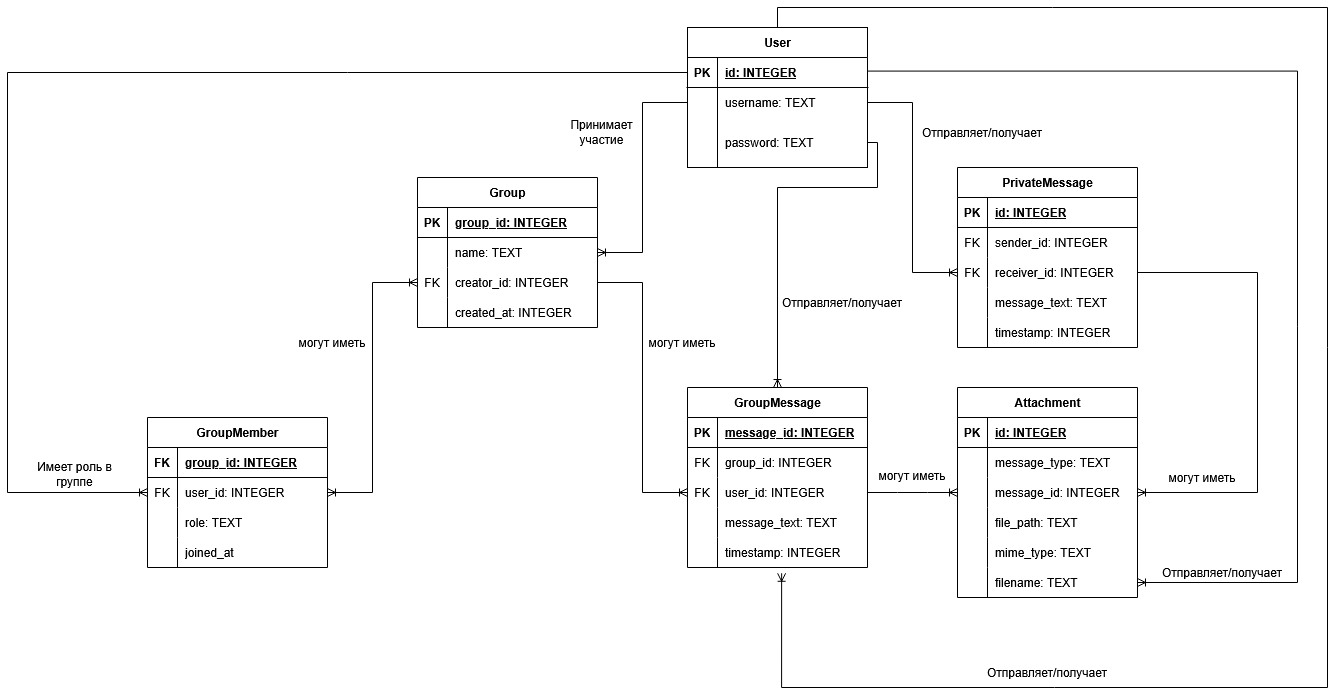
\includegraphics[width=1\linewidth]{ЕР модель}}
\caption{Диаграмма компонентов базы данных}
\label{comp:image}
\end{figure}

Диаграмма отражает логическую организацию таблиц, их назначение и ключевые взаимосвязи между ними.

\subsection{Таблицы базы данных}
\textbf{User - Пользователи системы}
\begin{xltabular}{\textwidth}{|l|l|X|}
	\caption{Атрибуты сущности "Пользователи"\label{user:table}}\\ \hline
	\centrow Поле & \centrow Тип & \centrow Описание \\ \hline
	\thead{id} & \thead{INTEGER} & Первичный ключ (PK), уникальный идентификатор пользователя \\ \hline
	\thead{username} & \thead{TEXT} & Имя пользователя (уникальное) \\ \hline
	\thead{password} & \thead{TEXT} & Хэшированный пароль пользователя \\ \hline
\end{xltabular}

Таблица "User" хранит информацию о зарегистрированных пользователях мессенджера. Каждый пользователь имеет уникальный идентификатор, имя пользователя и пароль. Является центральной сущностью системы, с которой связаны все остальные таблицы.

\textbf{Group - Групповые чаты}
\begin{xltabular}{\textwidth}{|l|l|X|}
	\caption{Атрибуты сущности "Групповые чаты"\label{group:table}}\\ \hline
	\centrow Поле & \centrow Тип & \centrow Описание \\ \hline
	\thead{group\_id} & \thead{INTEGER} & Первичный ключ (PK), ID группы \\ \hline
	\thead{name} & \thead{TEXT} & Название группы \\ \hline
	\thead{creator\_id} & \thead{INTEGER} & Внешний ключ (FK→User), ID создателя группы \\ \hline
	\thead{created\_at} & \thead{INTEGER} & Timestamp создания группы \\ \hline
\end{xltabular}

Таблица "Group" содержит информацию о групповых чатах. Каждая группа имеет уникальный идентификатор, название, создателя и время создания. Создатель группы автоматически становится владельцем (owner).

\textbf{GroupMember - Участники групп с ролями}
\begin{xltabular}{\textwidth}{|l|l|X|}
	\caption{Атрибуты сущности "Участники групп"\label{groupmember:table}}\\ \hline
	\centrow Поле & \centrow Тип & \centrow Описание \\ \hline
	\thead{group\_id} & \thead{INTEGER} & Внешний ключ (FK→Group), ID группы \\ \hline
	\thead{user\_id} & \thead{INTEGER} & Внешний ключ (FK→User), ID пользователя \\ \hline
	\thead{role} & \thead{TEXT} & Роль в группе: 'owner' (владелец), 'admin' (администратор), 'member' (участник) \\ \hline
	\thead{joined\_at} & \thead{INTEGER} & Timestamp вступления пользователя в группу \\ \hline
\end{xltabular}

Таблица "GroupMember" определяет состав участников групп и их роли. Реализует систему прав доступа, аналогичную Telegram, где владелец имеет максимальные права, администраторы - ограниченные права управления, а участники - базовые права.

\textbf{GroupMessage - Сообщения в группах}
\begin{xltabular}{\textwidth}{|l|l|X|}
	\caption{Атрибуты сущности "Групповые сообщения"\label{groupmessage:table}}\\ \hline
	\centrow Поле & \centrow Тип & \centrow Описание \\ \hline
	\thead{message\_id} & \thead{INTEGER} & Первичный ключ (PK), ID сообщения \\ \hline
	\thead{group\_id} & \thead{INTEGER} & Внешний ключ (FK→Group), ID группы \\ \hline
	\thead{user\_id} & \thead{INTEGER} & Внешний ключ (FK→User), ID отправителя \\ \hline
	\thead{message\_text} & \thead{TEXT} & Текст сообщения (может быть пустым для сообщений с вложениями) \\ \hline
	\thead{timestamp} & \thead{INTEGER} & Время отправки сообщения (timestamp) \\ \hline
\end{xltabular}

Таблица "GroupMessage" хранит все сообщения, отправленные в групповых чатах. Каждое сообщение связано с группой и пользователем-отправителем. Поддерживает текстовые сообщения и сообщения с вложениями (через таблицу Attachment).

\textbf{Attachment - Вложения к сообщениям}
\begin{xltabular}{\textwidth}{|l|l|X|}
	\caption{Атрибуты сущности "Вложения к сообщениям"\label{attachment:table}}\\ \hline
	\centrow Поле & \centrow Тип & \centrow Описание \\ \hline
	\thead{id} & \thead{INTEGER} & Первичный ключ (PK), уникальный идентификатор вложения \\ \hline
	\thead{message\_type} & \thead{TEXT} & Тип сообщения: 'general' (общее), 'group' (групповое), 'private' (личное) \\ \hline
	\thead{message\_id} & \thead{INTEGER} & Внешний ключ, ссылается на соответствующую таблицу сообщений \\ \hline
	\thead{file\_path} & \thead{TEXT} & Относительный путь к файлу в файловой системе сервера \\ \hline
	\thead{mime\_type} & \thead{TEXT} & MIME-тип файла (например, 'image/jpeg', 'application/pdf') \\ \hline
	\thead{filename} & \thead{TEXT} & Оригинальное имя файла при загрузке пользователем \\ \hline
\end{xltabular}

Таблица "Attachment" хранит информацию о файлах, прикреплённых к сообщениям. Каждая запись содержит метаданные файла и ссылку на сообщение, к которому он прикреплён. Файлы физически хранятся в файловой системе сервера, а в базе данных сохраняются только пути к ним. Поддерживаются вложения для всех типов сообщений (личные, групповые и общие).

\subsection{Диаграмма компонентов}

На рисунке \ref{data:image} представлена схема обмена данными между сценариями компонента при вызове компонента на странице сайта.

\begin{figure}[H]
\center{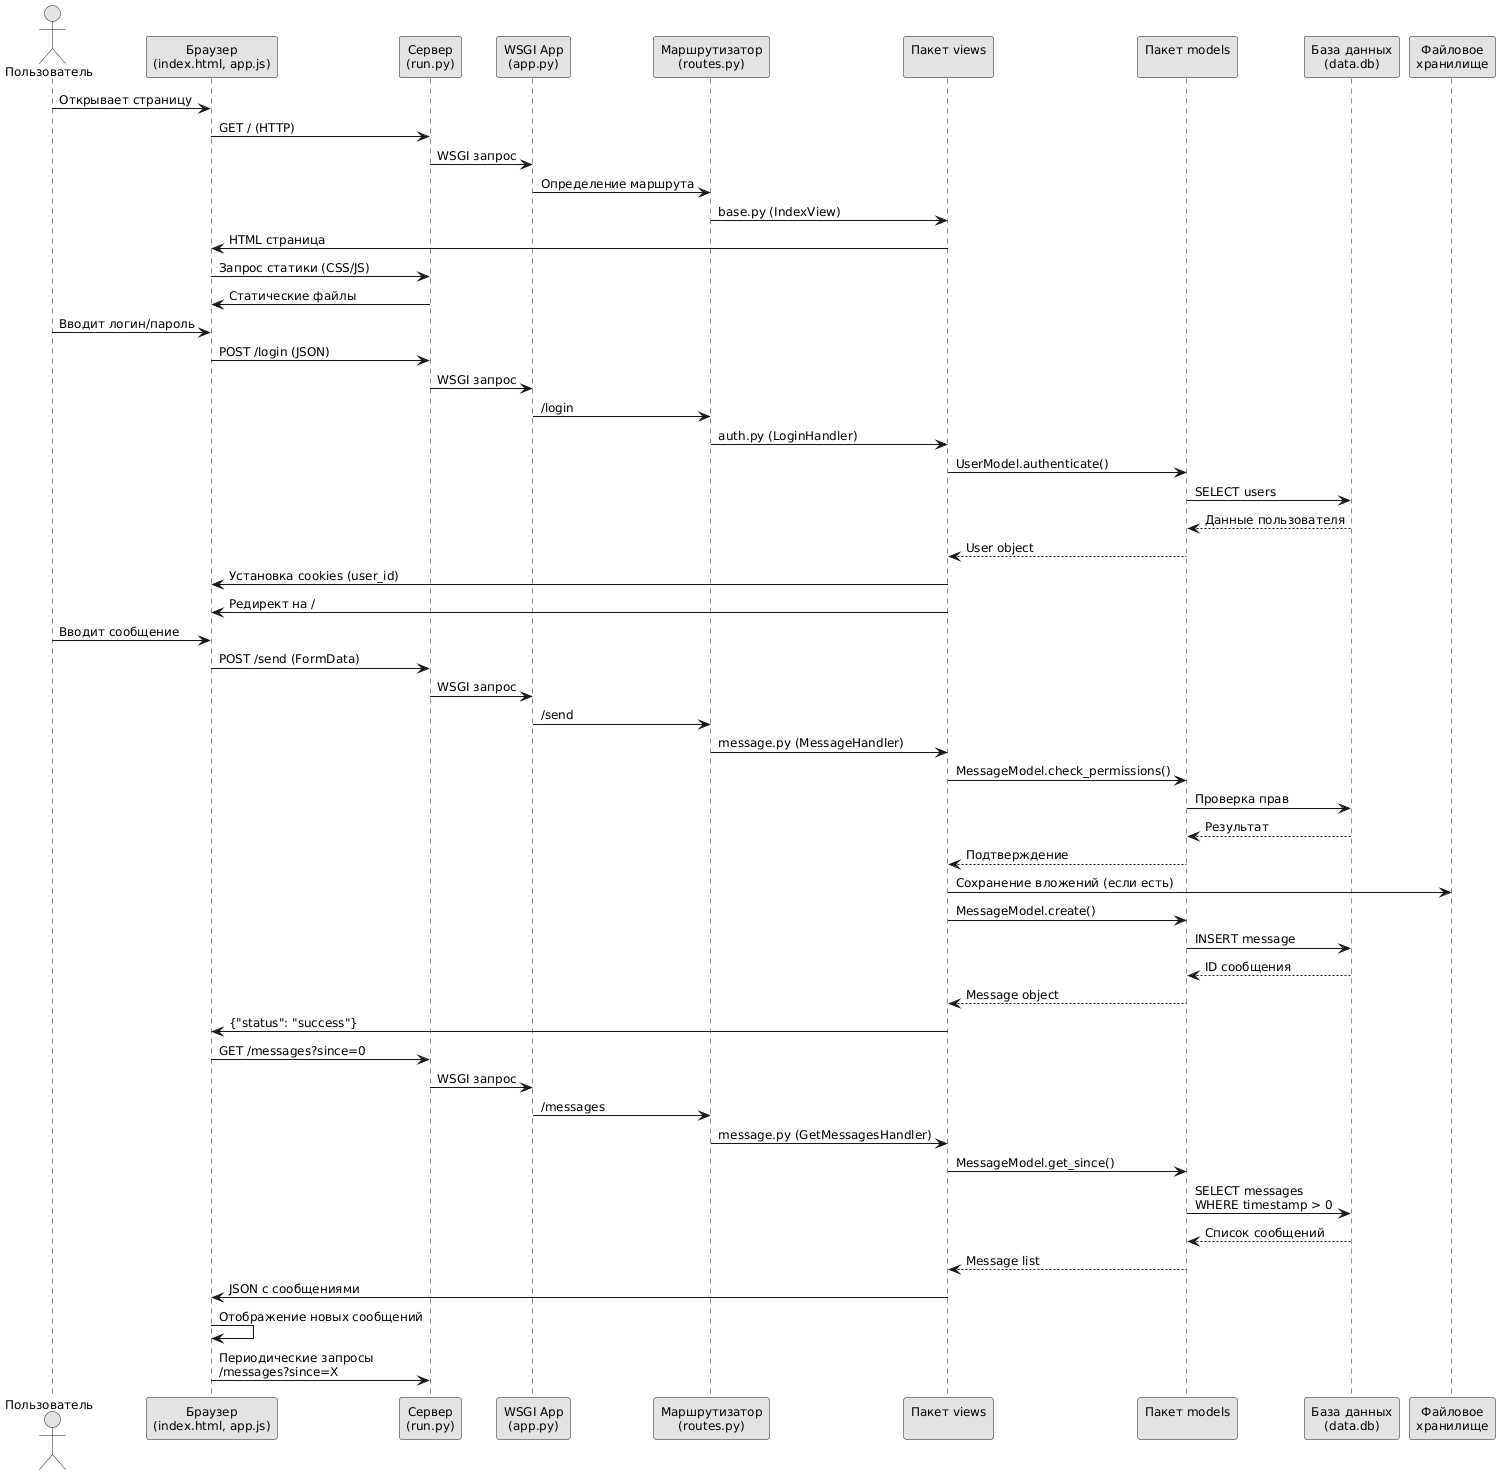
\includegraphics[width=1\linewidth]{Диаграмма последовательности}}
\caption{Диаграмма компонентов}
\label{data:image}
\end{figure}

\begin{enumerate}[leftmargin=*,label=\textbf{\arabic*.}]
	\item \textbf{Загрузка страницы (инициализация)}
	\begin{itemize}
		\item Пользователь открывает в браузере главную страницу (\texttt{index.html})
		\item Браузер отправляет HTTP GET-запрос на сервер
		\item Серверный скрипт \texttt{run.py} (Waitress) получает запрос
		\item Запрос передаётся в WSGI-приложение (\texttt{app.py})
		\item Маршрутизатор (\texttt{routes.py}) определяет обработчик \texttt{IndexView}
		\item Пользователю возвращается HTML-страница и статические файлы (CSS/JS)
	\end{itemize}
	
	\item \textbf{Процесс аутентификации}
	\begin{itemize}
		\item Пользователь вводит логин и пароль в форму входа
		\item Браузер отправляет POST /login запрос (JSON)
		\item \texttt{LoginView} проверяет учётные данные:
		\begin{itemize}
			\item Через \texttt{utils.py} выполняется SQL-запрос к таблице \texttt{users}
			\item Пароль проверяется с помощью bcrypt
		\end{itemize}
		\item При успешной аутентификации:
		\begin{itemize}
			\item Устанавливается cookie с \texttt{user\_id}
			\item Происходит редирект на главную страницу
		\end{itemize}
	\end{itemize}
	
	\item \textbf{Отправка нового сообщения}
	\begin{itemize}
		\item Пользователь вводит текст и/или прикрепляет файлы
		\item Браузер формирует FormData и отправляет POST /send\_message
		\item \texttt{SendMessageView} выполняет:
		\begin{itemize}
			\item Проверку прав через cookies
			\item Сохранение файлов в \texttt{static/uploads}
			\item Запись сообщения в БД (таблицы \texttt{messages} или \texttt{group\_messages})
		\end{itemize}
		\item Клиент получает JSON с результатом операции
	\end{itemize}
	
	\item \textbf{Получение сообщений (реализация чата)}
	\begin{itemize}
		\item Браузер периодически опрашивает сервер (GET /get\_messages)
		\item \texttt{GetMessageView} запрашивает новые сообщения из БД
		\item Сервер возвращает JSON с массивом сообщений
		\item Браузер динамически обновляет интерфейс чата
	\end{itemize}
	
	\item \textbf{Особенности работы}
	\begin{itemize}
		\item Все запросы проходят через единую точку входа (\texttt{app.py})
		\item Маршрутизатор выбирает соответствующий View-класс
		\item Бизнес-логика сосредоточена в \texttt{views.py}
		\item Работа с БД вынесена в \texttt{utils.py}
		\item Файлы хранятся локально в файловой системе
		\item Состояние сессии поддерживается через cookies
	\end{itemize}
\end{enumerate}

\subsection{Диаграмма размещения}

Диаграмма размещения (рис.~\ref{place:image}) отражает физические взаимосвязи между программными и аппаратными компонентами системы.

\begin{figure}[ht]
	\center{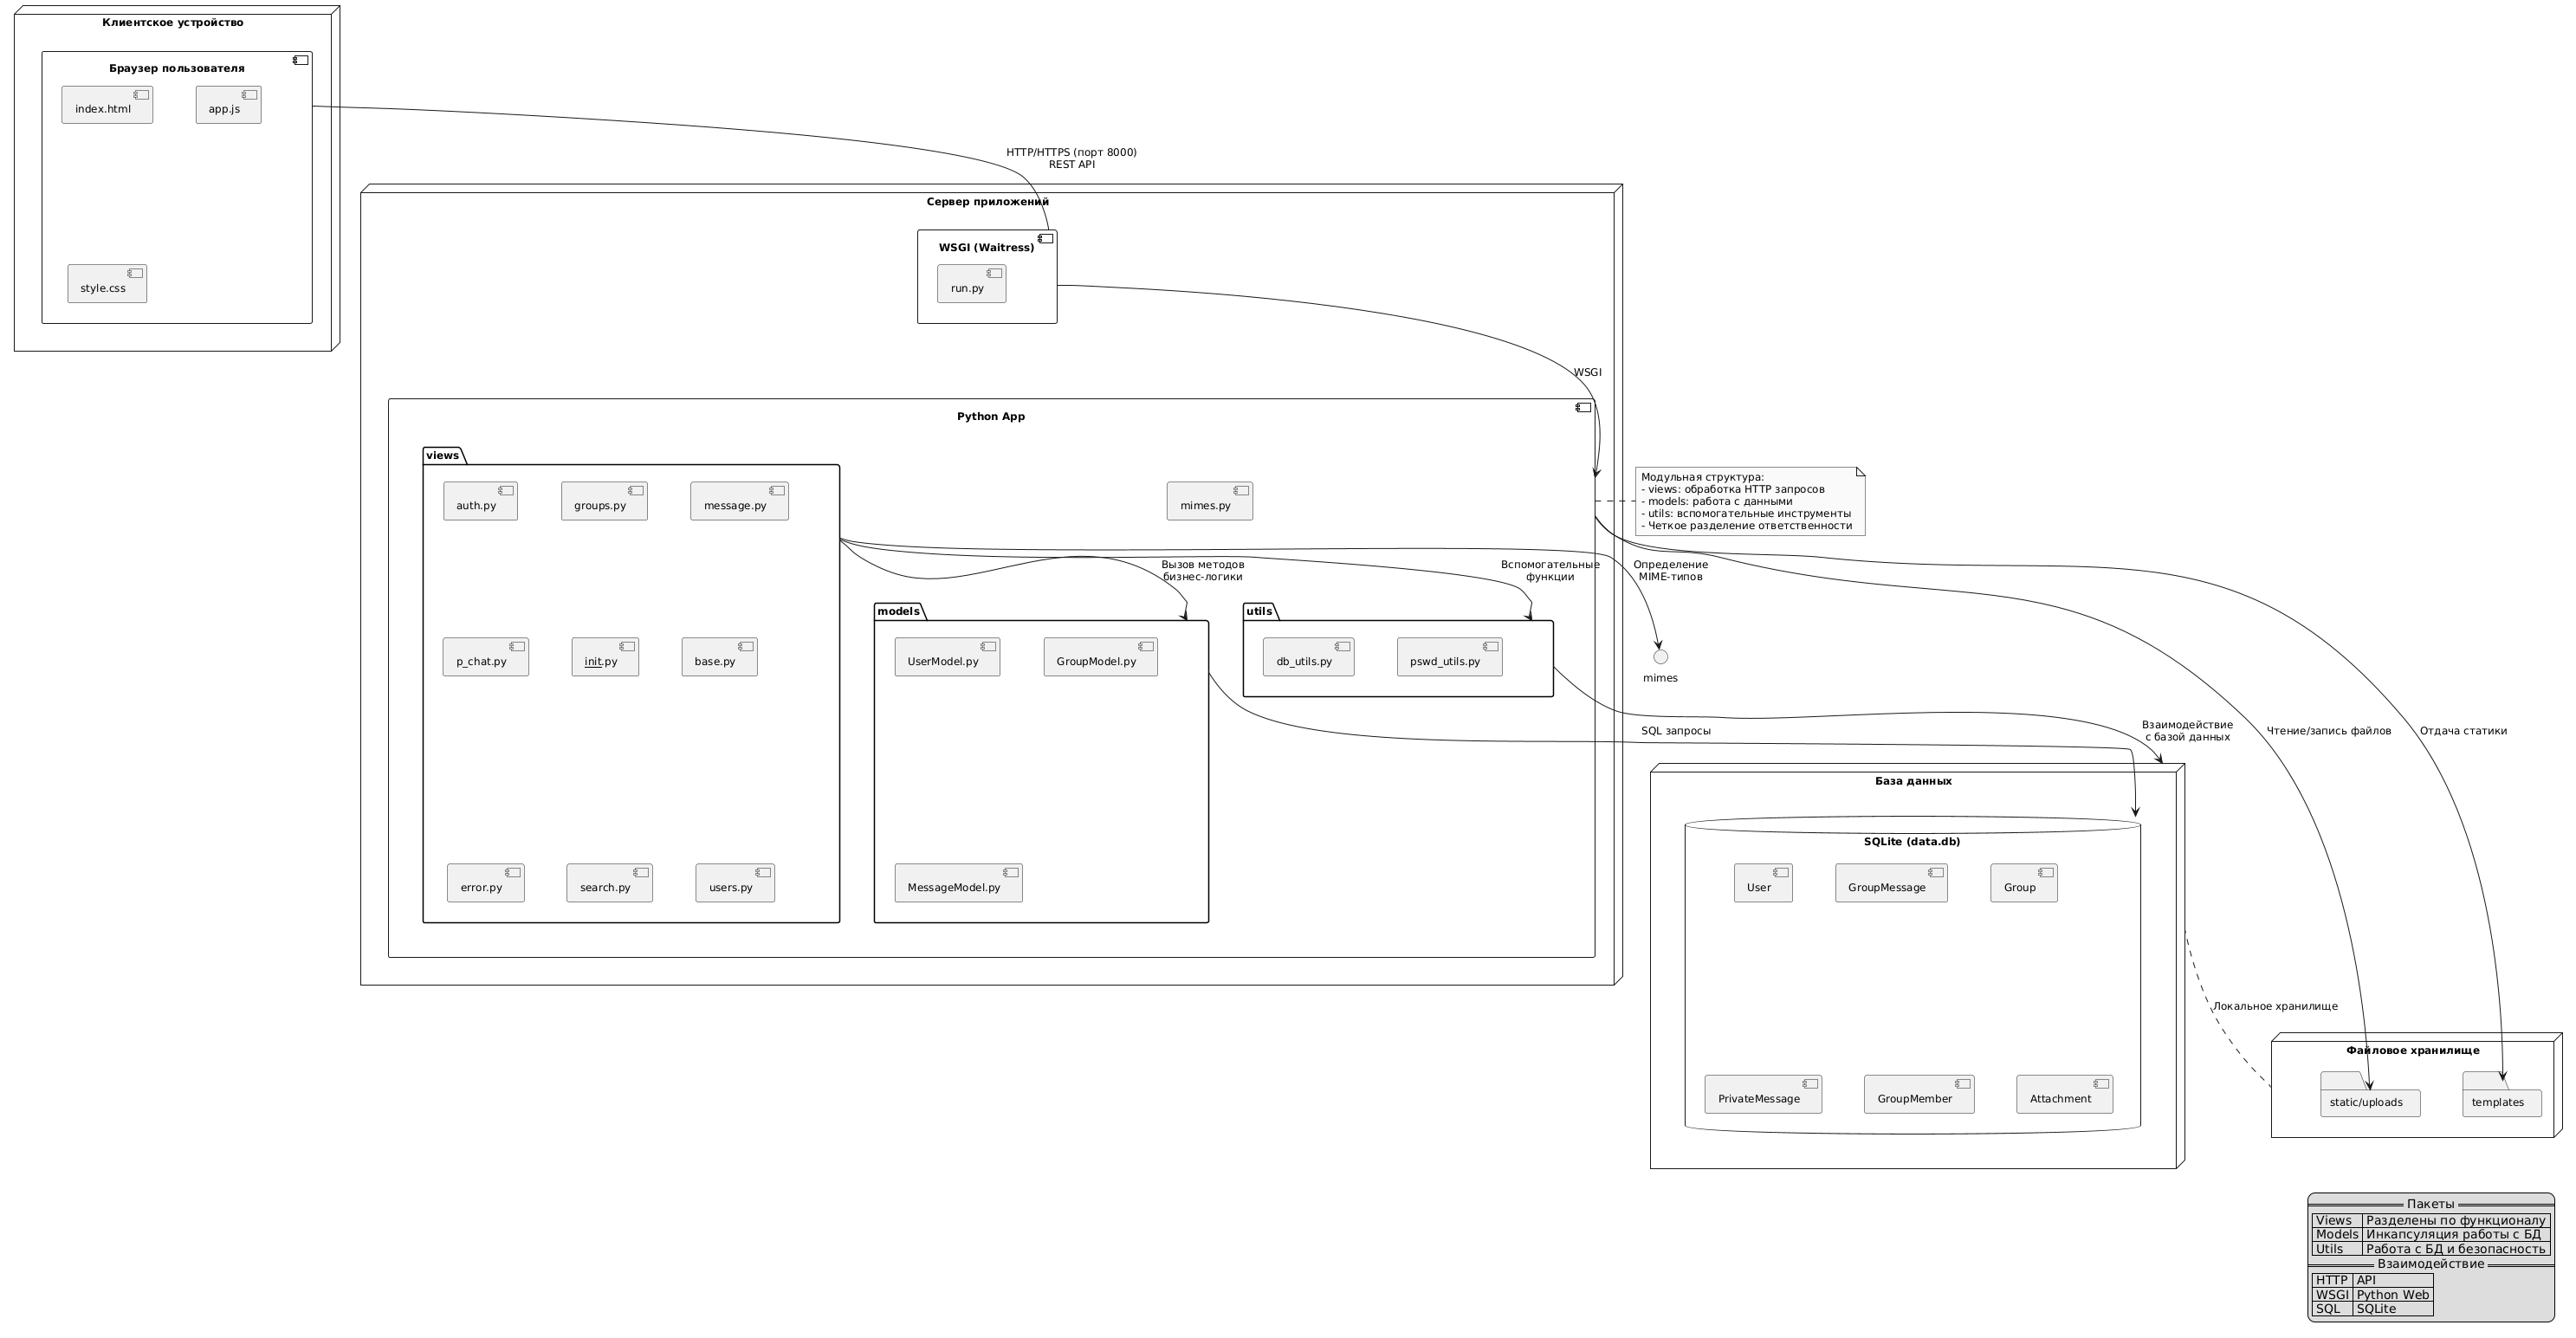
\includegraphics[width=1\linewidth]{Диаграмма развёртывания}}
	\caption{Диаграмма развёртывания}
	\label{place:image}
\end{figure}

Диаграмма развёртывания показывает физическую архитектуру системы, включая следующие ключевые компоненты:

\begin{itemize}
	\item \textbf{Клиентские устройства} - компьютеры и мобильные устройства пользователей с установленным веб-браузером
	\item \textbf{Веб-сервер} - серверное приложение на базе Waitress, обрабатывающее HTTP-запросы
	\item \textbf{WSGI-приложение} - ядро мессенджера, реализованное на Python с использованием Flask
	\item \textbf{База данных SQLite} - файл data.db, хранящий все данные системы
	\item \textbf{Файловое хранилище} - директория static/uploads для хранения прикреплённых файлов
\end{itemize}

Стрелки на диаграмме показывают направления взаимодействия между компонентами. Все клиенты взаимодействуют только с веб-сервером, который в свою очередь обращается к WSGI-приложению. Приложение работает с базой данных и файловым хранилищем.

	\ifПрактика{}\else{
		\section{Рабочий проект}
\subsection{Классы, используемые при разработке модели данных мессенджера}

\subsubsection{UserModel} 

Класс предназначен для управления данными пользователей. Он включает функционал для регистрации новых пользователей, аутентификации, поиска и получения информации о существующих аккаунтах.

\begin{xltabular}{\textwidth}{|l|X|}
	\caption{Методы класса UserModel}\\ \hline
	\centrow Метод & \centrow Описание \\ \hline
	authenticate & Выполняет проверку учетных данных пользователя. Запрашивает сохраненный хеш пароля и сравнивает его с введенным значением, возвращая ID пользователя при успешной проверке. \\ \hline
	create\_user & Добавляет нового пользователя в систему, выполняя проверку уникальности имени и хеширование пароля перед сохранением. \\ \hline
	get\_user\_by\_id & Возвращает учетные данные пользователя, включая его имя, если найден соответствующий ID. \\ \hline
	get\_user\_id & Ищет пользователя в базе данных по имени и возвращает его ID. \\ \hline search\_users & Выполняет поиск пользователей по частичному совпадению имени. Позволяет исключать текущего пользователя из результатов поиска. \\ \hline
\end{xltabular}

\subsubsection{MessageModel} 

Класс отвечает за управление сообщениями в системе, позволяя пользователям отправлять, редактировать и удалять сообщения. Поддерживается работа как с личными, так и групповыми чатами, а также вложениями.

\begin{xltabular}{\textwidth}{|l|X|}
	\caption{Методы класса MessageModel}\\ \hline
	\centrow Метод & \centrow Описание \\ \hline
	get\_general\_messages & Возвращает сообщения общего чата, загружая только те, которые были отправлены после указанной временной метки. \\ \hline
	get\_group\_messages & Извлекает сообщения группового чата, принадлежащие указанной группе, начиная с заданного времени. \\ \hline
	get\_private\_messages & Загружает приватные сообщения между двумя пользователями, отфильтрованные по временной метке. \\ \hline
	create\_message & Создает сообщение соответствующего типа (общее, групповое или приватное). Определяет отправителя и сохраняет данные в базе. \\ \hline
	edit\_message & Позволяет пользователю изменить содержимое ранее отправленного сообщения, проверяя права доступа перед внесением изменений. \\ \hline
	delete\_message & Удаляет сообщение из базы данных. Проверяет, имеет ли пользователь право на удаление, прежде чем выполнить операцию. \\ \hline
	search\_messages & Выполняет поиск сообщений по заданному текстовому запросу, фильтруя результаты по типу чата и пользователю. \\ \hline
	add\_attachment & Прикрепляет файл к определенному сообщению, сохраняя его путь, MIME-тип и оригинальное имя. \\ \hline
\end{xltabular}

\subsubsection{GroupModel}

Класс предоставляет функционал для управления группами, в том числе создание новых чатов, добавление и удаление участников, а также настройку ролей пользователей в группе.

\begin{xltabular}{\textwidth}{|l|X|}
	\caption{Методы класса GroupModel}\\ \hline
	\centrow Метод & \centrow Описание \\ \hline
	create\_group & Создает новую группу с заданным именем и указывает её владельца. \\ \hline 
	\_group & Позволяет владельцу или администратору изменить название группы. \\ \hline 
	\_member & Добавляет нового участника в группу и назначает ему роль (владелец, администратор или участник). \\ \hline
	remove\_member & Исключает пользователя из группы, проверяя права инициатора удаления. \\ \hline
	change\_role & Меняет роль участника в группе, например, повышая до администратора. \\ \hline
	get\_group\_members & Возвращает список всех участников группы, включая их роли и дату присоединения. \\ \hline
	check\_group\_access & Проверяет, является ли пользователь участником группы и обладает ли правами доступа. \\ \hline
\end{xltabular}

\subsubsection{get\_db\_cursor}

Контекстный менеджер, предназначенный для управления подключением к базе данных. Позволяет автоматически открывать и закрывать курсор, предотвращая утечки соединений.

\begin{xltabular}{\textwidth}{|l|X|}
	\caption{Методы класса get\_db\_cursor}\\ \hline
	\centrow Метод & \centrow Описание \\ \hline
	enter & Открывает соединение с базой данных и создает объект курсора. \\ \hline
	exit & Закрывает курсор и соединение при выходе из контекста. \\ \hline
\end{xltabular}

\subsection{Модульное тестирование разработанного web-сайта}

Модульный тест для класса User из модели данных представлен на рисунке \ref{unitUser:image}.

\begin{figure}[ht]
\begin{lstlisting}[language=Python]
from django.test import TestCase
from .models import *
User = get_user_model()


class ShpoTestCases(TestCase):

    def setUp(self) -> None:
        self.user = User.objects.create(username='testtestovich', password='testtestovich', first_name='Sad', last_name='')

    def test_2(self):

        self.assertEqual(self.user.first_name, 'Sad')
        self.assertEqual(self.user.last_name, 'Cat')
        print((self.user))
        print((self.user.first_name))
        print((self.user.last_name))
\end{lstlisting}  
\caption{Модульный тест класса User}
\label{unitUser:image}
\end{figure}

\subsection{Системное тестирование разработанного web-сайта}

На рисунке \ref{main:image} представлена главная страница сайта «Русатом – Аддитивные технологии».
\newpage % при необходимости можно переносить рисунок на новую страницу
\begin{figure}[H] % H - рисунок обязательно здесь, или переносится, оставляя пустоту
\center{\includegraphics[width=1\linewidth]{main1}}
\center{\includegraphics[width=1\linewidth]{main2}}
\center{\includegraphics[width=1\linewidth]{main3}}
\caption{Главная страница сайта «Русатом – Аддитивные технологии»}
\label{main:image}
\end{figure}

На рисунке \ref{menu:image} представлен динамический вывод заголовков, включающий в себя искомые фразы при поиске фраз.

\begin{figure}[ht]
\center{\includegraphics[width=1\linewidth]{menu}}
\caption{Динамический вывод заголовков}
\label{menu:image}
\end{figure}

На рисунке \ref{enter:image} представлен ввод данных для публикации новости.

\begin{figure}[ht]
\center{\includegraphics[width=1\linewidth]{enter}}
\caption{Ввод данных для публикации очень-очень длинной, интересной и полезной новости}
\label{enter:image}
\end{figure}

		\section*{ЗАКЛЮЧЕНИЕ}
\addcontentsline{toc}{section}{ЗАКЛЮЧЕНИЕ}

Преимущества аддитивных технологий заключается в разнообразии процессов, позволяющих применять их в различных областях производства. Существенным ограничением же является и экономическая составляющая, которая не позволит внедрить аддитивное производство повсеместно.
  
Компании, видя, как развиваются информационные технологии, пытаются использовать их выгодно для своего бизнеса, запуская свой сайт для того, чтобы заявить о своем существовании, проинформировать потенциального клиента об услугах или продуктах, которые предоставляет. 
Для продвижения компании «Русатом – Аддитивные технологии» был разработан веб-сайт на основе системы «1С-Битрикс: Управление сайтом».

Основные результаты работы:

\begin{enumerate}
\item Проведен анализ предметной области. Выявлена необходимость использовать 1С-Битрикс.
\item Разработана концептуальная модель web-сайта. Разработана модель данных системы. Определены требования к системе.
\item Осуществлено проектирование web-сайта. Разработана архитектура серверной части. Разработан пользовательский интерфейс web-сайта.
\item Реализован и протестирован web-сайт. Проведено модульное и системное тестирование.
\end{enumerate}

Все требования, объявленные в техническом задании, были полностью реализованы, все задачи, поставленные в начале разработки проекта, были также решены.

Готовый рабочий проект представлен адаптивной версткой сайта. Сайт находится в публичном доступе, поскольку опубликован в сети Интернет.  

	}\fi
	\addcontentsline{toc}{section}{СПИСОК ИСПОЛЬЗОВАННЫХ ИСТОЧНИКОВ}

\begin{thebibliography}{9}
	
	\bibitem{abramov} Абрамов, С. М. Python: создание веб-сайтов / С. М. Абрамов. – Москва~: Эксмо, 2020. – 320 с. – ISBN 978-5-04-109098-2. – Текст~: непосредственный.
	
	\bibitem{brown} Браун, Э. Python и анализ данных / Э. Браун. – Санкт-Петербург~: БХВ-Петербург, 2019. – 400 с. – ISBN 978-5-9775-4105-3. – Текст~: непосредственный.
	
	\bibitem{vasiliev} Васильев, А. Н. Python на примерах. Практический курс по программированию / А. Н. Васильев. – Санкт-Петербург~: Наука и Техника, 2017. – 432 с. – ISBN 978-5-94387-982-6. – Текст~: непосредственный.
	
	\bibitem{golub} Голубь, Н. Python. Основы программирования / Н. Голубь. – Санкт-Петербург~: Питер, 2021. – 416 с. – ISBN 978-5-4461-1431-9. – Текст~: непосредственный.
	
	\bibitem{zlatopolsky} Златопольский, Д. М. Основы программирования на языке Python / Д. М. Златопольский. – Москва~: ДМК Пресс, 2021. – 288 с. – ISBN 978-5-97060-873-1. – Текст~: непосредственный.
	
	\bibitem{lukin} Лукин, С. Н. Разработка веб-приложений на Python с использованием фреймворка Flask / С. Н. Лукин. – Москва~: БИНОМ. Лаборатория знаний, 2018. – 288 с. – ISBN 978-5-9963-3580-9. – Текст~: непосредственный.
	
	\bibitem{mckinley} Маккинли, У. Python и обработка данных / У. Маккинли. – Москва~: ДМК Пресс, 2016. – 482 с. – ISBN 978-5-97060-392-7. – Текст~: непосредственный.
	
	\bibitem{muller} Мюллер, Дж. Python для чайников / Дж. Мюллер. – Москва~: Диалектика, 2019. – 416 с. – ISBN 978-5-907114-25-3. – Текст~: непосредственный.
	
	\bibitem{ramalho} Рамальо, Л. Python. К вершинам мастерства / Л. Рамальо. – Москва~: ДМК Пресс, 2016. – 768 с. – ISBN 978-5-97060-384-2. – Текст~: непосредственный.
	
	\bibitem{reitz} Рейтц, К. Разработка Web API на Python / К. Рейтц, Т. Шахэм. – Санкт-Петербург~: Питер, 2014. – 272 с. – ISBN 978-5-496-01153-2. – Текст~: непосредственный.
	
	\bibitem{sedlacek} Седлачек, Р. Django 3. Практика создания современных Web-приложений / Р. Седлачек. – Санкт-Петербург~: БХВ-Петербург, 2021. – 416 с. – ISBN 978-5-9775-0661-8. – Текст~: непосредственный.
	
	\bibitem{simonov} Симонов, М. Python. Самое необходимое / М. Симонов. – Санкт-Петербург~: БХВ-Петербург, 2020. – 320 с. – ISBN 978-5-9775-0647-2. – Текст~: непосредственный.
	
	\bibitem{stevenson} Стивенсон, Т. Python. Самоучитель / Т. Стивенсон. – Москва~: ДМК Пресс, 2017. – 322 с. – ISBN 978-5-97060-510-5. – Текст~: непосредственный.
	
	\bibitem{fedorov} Федоров, Д. Ю. Программирование на языке Python / Д. Ю. Федоров. – Москва~: БИНОМ. Лаборатория знаний, 2019. – 224 с. – ISBN 978-5-9963-3581-6. – Текст~: непосредственный.
	
	\bibitem{chernyshev} Чернышев, А. Python. Исчерпывающее руководство / А. Чернышев. – Санкт-Петербург~: БХВ-Петербург, 2018. – 512 с. – ISBN 978-5-9775-3898-5. – Текст~: непосредственный.
	
\end{thebibliography}
	\ifВКР{\appendix{Представление графического материала}

Графический материал, выполненный на отдельных листах,
изображен на рисунках А.1--А.\arabic{числоПлакатов}.
\setcounter{числоПлакатов}{0}

\renewcommand{\thefigure}{А.\arabic{figure}} % шаблон номера для плакатов

\begin{landscape}

\begin{плакат}
    
\includegraphics[width=0.82\linewidth]{плакат1.png}
    \заголовок{Сведения о ВКРБ}
    \label{pl1:image}      
\end{плакат}

\begin{плакат}
    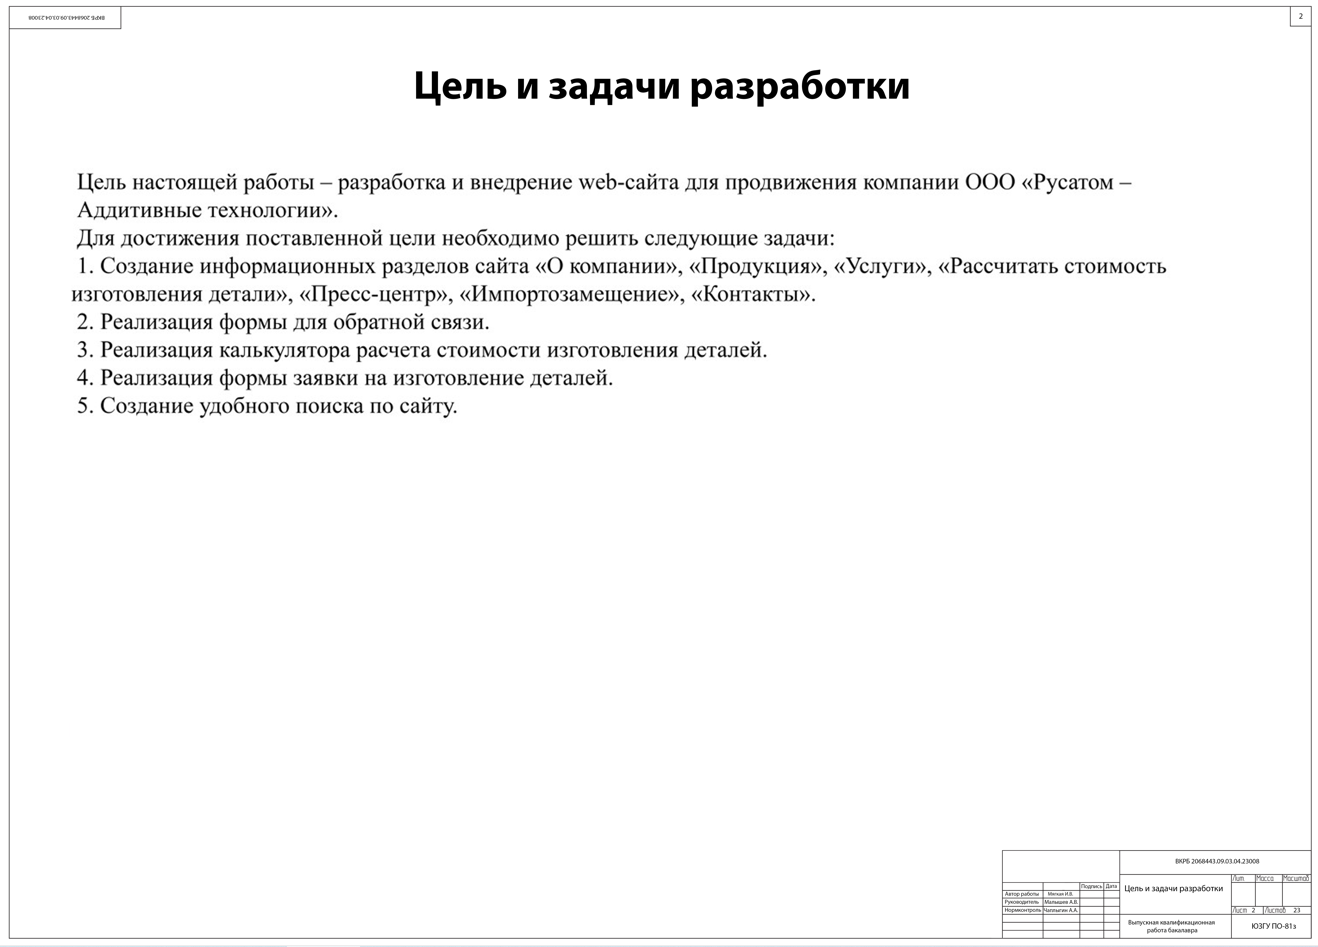
\includegraphics[width=0.82\linewidth]{плакат2.png}
    \заголовок{Цель и задачи разработки}
    \label{pl2:image}      
\end{плакат}

\begin{плакат}
    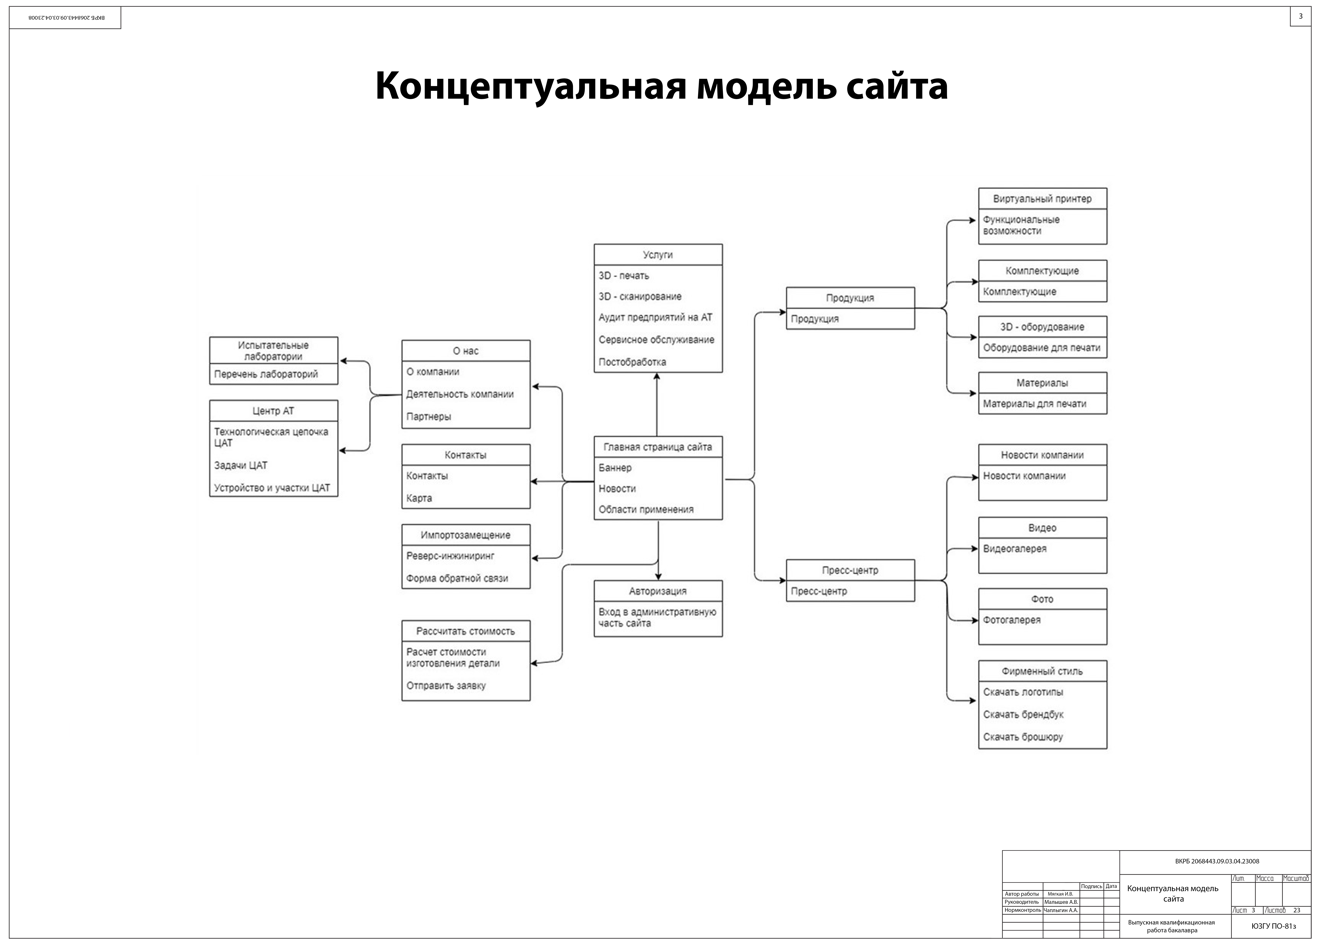
\includegraphics[width=0.82\linewidth]{плакат3.png}
    \заголовок{Концептуальная модель сайта}
    \label{pl3:image}      
\end{плакат}

\begin{плакат}
    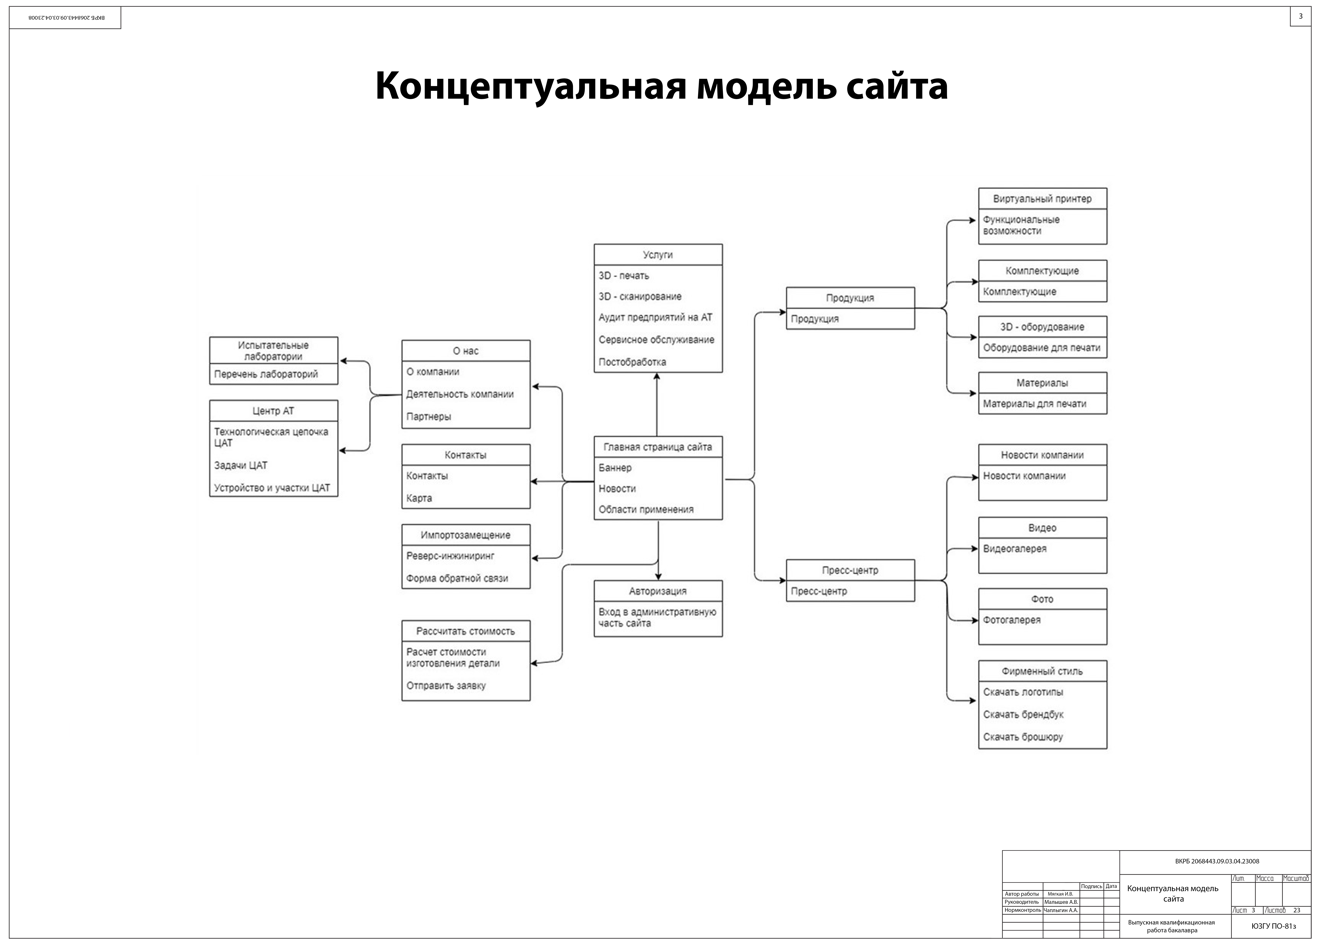
\includegraphics[width=0.82\linewidth]{плакат3.png}
    \заголовок{Еще плакат}
    \label{pl4:image}      
\end{плакат}

\end{landscape}
}\fi
	\ifПрактика{}\else{\appendix{Фрагменты исходного кода программы}

main.tex
\lstinputlisting[language=Tex, frame=none]{main.tex}

ТехПроект.tex
\lstinputlisting[language=Tex, frame=none]{ТехПроект.tex}

\ifВКР{
\newpage
\addcontentsline{toc}{section}{На отдельных листах (CD-RW в прикрепленном конверте)}
\noindent
\begin{tabular}{p{5.8cm}C{4.8cm}C{4.8cm}}
   Автор ВКР & \lhrulefill{\fill} & \fillcenter\Автор \\
            \setarstrut{\footnotesize}
           & \footnotesize{(подпись, дата)} & \\
            \restorearstrut
   Руководитель ВКР & \lhrulefill{\fill} & \fillcenter\Руководитель \\
            \setarstrut{\footnotesize}
           & \footnotesize{(подпись, дата)} & \\
            \restorearstrut
   Нормоконтроль & \lhrulefill{\fill} & \fillcenter\Нормоконтроль \\
            \setarstrut{\footnotesize}
           & \footnotesize{(подпись, дата)} & \\
            \restorearstrut
\end{tabular}
\vskip 2cm
\begin{center}
\textbf{Место для диска}
\end{center}
}\fi
}\fi
\end{document}
